% main.tex, to be used with thesis.tex
% This contains the main work of your thesis.

%\bibliography{thesis}  % uses the references stored in Chapter1Radar.bib

\chapter{Taxonomic Classification of Data Persistence in Sensor Networks}
\label{chap:taxonomies}

Different mechanisms are used for persisting data collected from sensor
networks, as described by the section regarding the state of the art in sensor
networks and different approaches for persistence. This section analyzes these
approaches and presents the different approaches through
taxonomy\footnote{Taxonomy is the practice and science of classification, by
using taxonomic units known as taxa (singular taxon)}, which were used
throughout this work to evaluate different existing database systems
implementations, taking into account different requirements and specifications
of different sensor networks.

\section{Purpose of the Sensor Data Taxonomy}

No matter the resource management used, the first taxonomy presented relates to
the purpose of the use of the collected sensor data. That is, when and how the
collected data is going to be used as described in section
\ref{sec:sn-data-purpose}.

\begin{figure}[h]
  \centering
  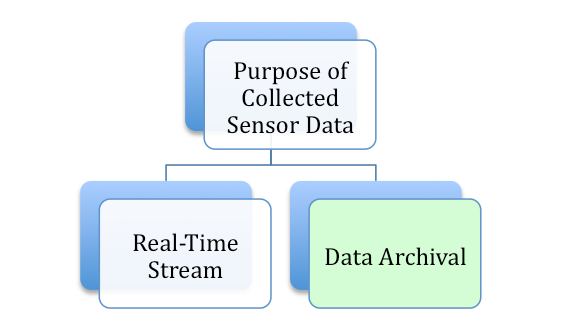
\includegraphics{../diagrams/taxonomy-data-purpose}
  \caption{The Purpose of Sensor Data Taxonomy}
  \label{fig:taxonomy-data-purpose}
\end{figure}

\begin{itemize}
  \item \textbf{Real-time Data Stream}: data is used as real-time data stream
  during data query \cite{sn-intro01};
  \item \textbf{Archival Data}: data is used for historical purposes such as
  data analysis or data fusion \cite{sn-intro01, sn-intro02}.
\end{itemize}

\section{The Location of the Sensor Data Taxonomy}

Directly related to the purpose of data, the procedure for data storage
described in section \ref{sec:sn-infrastructure} depends on the purpose of the
use of the collected data. Figure \ref{fig:taxonomy-data-location}, shows the
related taxon and can be described as follows:

\begin{figure}[h]
  \centering
  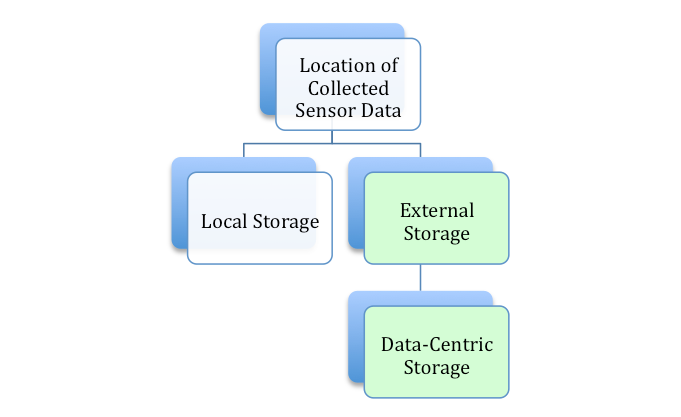
\includegraphics{../diagrams/taxonomy-data-location}
  \caption{The Location of Sensor Data Taxonomy}
  \label{fig:taxonomy-data-location}
\end{figure}

\begin{itemize}
  \item \textbf{Local Storage}: The data can be persisted in a temporarily
  memory address, or a secondary memory device in a local storage device. It is
  directly related to the real-time data stream taxon, since it occurs at the
  place of the sensor device;
  \item \textbf{External Storage}: The data is usually located in an external
  storage devicewith a data management system such as a database system;
  \item \textbf{Data-Centric Storage}:the collected data can organized in a
  categorizedmanner as described by \cite{sn-storage03}. This taxon regarding
  the system allows the data to bepartitioned by a particular property.
  Nowadays, this strategy is often related to database partition
  \cite{db-partition}, and database sharding approaches \cite{db-shard-intro,
  db-shard-discussion}.
\end{itemize}

\section{Data Model Taxonomy}

One of the fundamental challenges in the development of a persistence storage
in sensor network is related to the data model chosen to keep the collected
data. The introduction of new sensor devices may cause refactoring of the
existing model or not, depending on how the data model accommodates the data.
Different data models are reported to be used in the literature, as described
in section \ref{sec:data-models}. For this reason, taxonomy related to the
data model depicts two different classes of data models, as shown in Figure
\ref{fig:taxonomy-data-model}.

\begin{figure}[h]
  \centering
  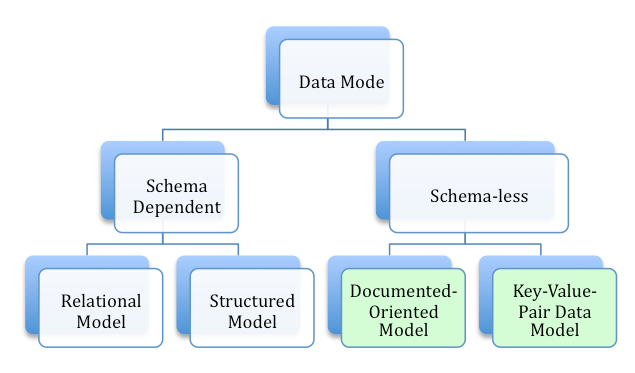
\includegraphics{../diagrams/taxonomy-data-model}
  \caption{Data Model Taxonomy}
  \label{fig:taxonomy-data-model}
\end{figure}

\begin{itemize}
  \item \textbf{Schema-Dependent Models}: this data model requires the
  definitionof a master schema that describes the data through a rigorous data
  modeling process prior to the use of the data. In addition, an addition to a
  newsensor device, and hence a new data entity, requires a re-evaluation ofthe
  existing data schema. For example, relational model is governed by
  therelational algebra model \cite{relational-model}, while the structured
  models such as XML \cite{xml} needs adefinition of an XML Schema
  \cite{xml-schema};
  \item \textbf{Schema-less Models}: contrary to the former taxon, schema-less
  data models do not require the definition of a data schema or a master table
  definition, along with its table relationships, if necessary. Instances of
  such data model is the Key-Value Pair \cite{db-kvp} and its variation
  document-oriented models \cite{db-is-rdbs-dommed}, whose use in wireless
  sensor networks has not been reported.
\end{itemize}

\section{Data Provenance Taxonomy}

No matter the data model used, the support for Data Provenance as shown in
section \ref{sec:sn-provenance} is as valuable as the data being collected.
For this reason, the data model taxonomy must have support for the data types
that support the use of provenance-related attributes in the collected sensor
data. In this way, Figure \ref{fig:taxonomy-data-provenance} describes the
data types for the metadata support.

\begin{figure}[h]
  \centering
  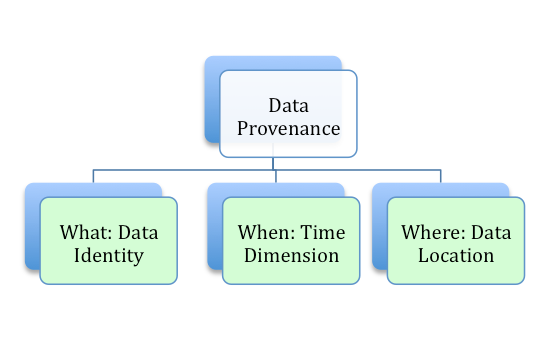
\includegraphics{../diagrams/taxonomy-data-provenance}
  \caption{Data Provenance Taxonomy}
  \label{fig:taxonomy-data-provenance}
\end{figure}

\begin{itemize}
  \item \textbf{What: Data Identity}: the data type that uniquely identifies
  the collected sensor data;
  \item \textbf{When: Time Dimension}: the data type that identifies the
  collected data;
  \item \textbf{Where: Data Location}: an optional data type that identifies
  from where the data originated.
\end{itemize}

\section{Query Processing Mechanism Taxonomy}

The query processing mechanism in sensor networks is directly related to how
and where the collected data is used and stored, as shown in the previous
section. As a consequence, the following taxonomy taxon is related to the
different types of query processing mechanisms described in section
\ref{sec:query-process}, and can be seen in Figure
\ref{fig:taxonomy-query-mechanism}.

\begin{figure}[h]
  \centering
  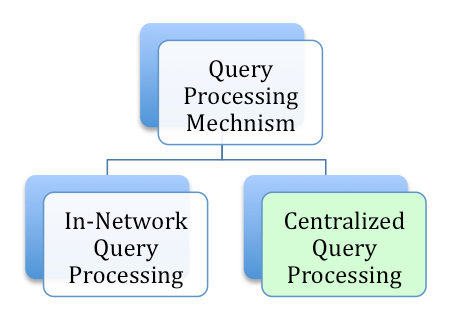
\includegraphics{../diagrams/taxonomy-query-mechanism}
  \caption{Query Processing Mechanism Taxonomy}
  \label{fig:taxonomy-query-mechanism}
\end{figure}

\begin{itemize}
  \item \textbf{In-Network Query Processing}: the sensor node receives a
  request to theproperties of the sensor, and returns the current values
  related to them \cite{sn-intro01};
  \item \textbf{Centralized Query Processing}: as developed in single server
  relational databases, the data is collected to a centralized data sink in
  order to be used.
\end{itemize}

\section{Database System Organization Taxonomy}

Different approaches of data storage can also be related to the performance in
the database system used, and how its architecture provides the data storage
solution. For example, one crucial problem related to the centralized network
sink in sensor networks is the presence of an ineluctable develoment of a point
of traffic concentration at this node \cite{sn-storage02}. In this way, in
order to reduce the problems associated with the so-called ``Funneling Effect",
Figure \ref{fig:taxonomy-database-architecture} summarizes the different
capabilities of different types of database systems.

\begin{figure}[h]
  \centering
  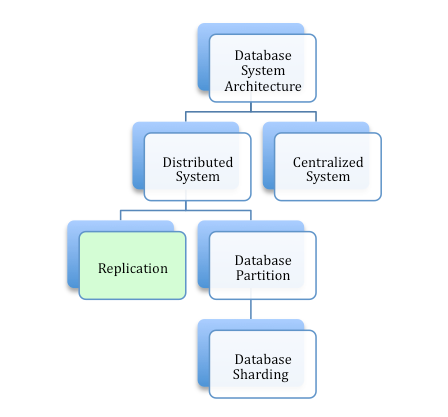
\includegraphics{../diagrams/taxonomy-database-architecture}
  \caption{Database Architecture Taxonomy}
  \label{fig:taxonomy-database-architecture}
\end{figure}

\begin{itemize}
  \item \textbf{Centralized System}: a database system that runs in one single
  centralized host, being the focal purpose of data traffic as read and writes 
  \cite{sn-intro01};
  \item \textbf{Distributed System}: a database system that can be composed by
  more thanone node. Usually, the use of the pattern of Master-Slave
  mechanisms can beused by implementing ``Replication". In addition to it,
  ``Database Sharding" is used to portion the data related to a given shard key.
\end{itemize}